% Options for packages loaded elsewhere
\PassOptionsToPackage{unicode}{hyperref}
\PassOptionsToPackage{hyphens}{url}
%
\documentclass[
]{article}
\usepackage{amsmath,amssymb}
\usepackage{lmodern}
\usepackage{ifxetex,ifluatex}
\ifnum 0\ifxetex 1\fi\ifluatex 1\fi=0 % if pdftex
  \usepackage[T1]{fontenc}
  \usepackage[utf8]{inputenc}
  \usepackage{textcomp} % provide euro and other symbols
\else % if luatex or xetex
  \usepackage{unicode-math}
  \defaultfontfeatures{Scale=MatchLowercase}
  \defaultfontfeatures[\rmfamily]{Ligatures=TeX,Scale=1}
\fi
% Use upquote if available, for straight quotes in verbatim environments
\IfFileExists{upquote.sty}{\usepackage{upquote}}{}
\IfFileExists{microtype.sty}{% use microtype if available
  \usepackage[]{microtype}
  \UseMicrotypeSet[protrusion]{basicmath} % disable protrusion for tt fonts
}{}
\makeatletter
\@ifundefined{KOMAClassName}{% if non-KOMA class
  \IfFileExists{parskip.sty}{%
    \usepackage{parskip}
  }{% else
    \setlength{\parindent}{0pt}
    \setlength{\parskip}{6pt plus 2pt minus 1pt}}
}{% if KOMA class
  \KOMAoptions{parskip=half}}
\makeatother
\usepackage{xcolor}
\IfFileExists{xurl.sty}{\usepackage{xurl}}{} % add URL line breaks if available
\IfFileExists{bookmark.sty}{\usepackage{bookmark}}{\usepackage{hyperref}}
\hypersetup{
  pdftitle={MATH 629 HW 4 Solutions},
  pdfauthor={Drew Lazar},
  hidelinks,
  pdfcreator={LaTeX via pandoc}}
\urlstyle{same} % disable monospaced font for URLs
\usepackage[margin=1in]{geometry}
\usepackage{color}
\usepackage{fancyvrb}
\newcommand{\VerbBar}{|}
\newcommand{\VERB}{\Verb[commandchars=\\\{\}]}
\DefineVerbatimEnvironment{Highlighting}{Verbatim}{commandchars=\\\{\}}
% Add ',fontsize=\small' for more characters per line
\usepackage{framed}
\definecolor{shadecolor}{RGB}{248,248,248}
\newenvironment{Shaded}{\begin{snugshade}}{\end{snugshade}}
\newcommand{\AlertTok}[1]{\textcolor[rgb]{0.94,0.16,0.16}{#1}}
\newcommand{\AnnotationTok}[1]{\textcolor[rgb]{0.56,0.35,0.01}{\textbf{\textit{#1}}}}
\newcommand{\AttributeTok}[1]{\textcolor[rgb]{0.77,0.63,0.00}{#1}}
\newcommand{\BaseNTok}[1]{\textcolor[rgb]{0.00,0.00,0.81}{#1}}
\newcommand{\BuiltInTok}[1]{#1}
\newcommand{\CharTok}[1]{\textcolor[rgb]{0.31,0.60,0.02}{#1}}
\newcommand{\CommentTok}[1]{\textcolor[rgb]{0.56,0.35,0.01}{\textit{#1}}}
\newcommand{\CommentVarTok}[1]{\textcolor[rgb]{0.56,0.35,0.01}{\textbf{\textit{#1}}}}
\newcommand{\ConstantTok}[1]{\textcolor[rgb]{0.00,0.00,0.00}{#1}}
\newcommand{\ControlFlowTok}[1]{\textcolor[rgb]{0.13,0.29,0.53}{\textbf{#1}}}
\newcommand{\DataTypeTok}[1]{\textcolor[rgb]{0.13,0.29,0.53}{#1}}
\newcommand{\DecValTok}[1]{\textcolor[rgb]{0.00,0.00,0.81}{#1}}
\newcommand{\DocumentationTok}[1]{\textcolor[rgb]{0.56,0.35,0.01}{\textbf{\textit{#1}}}}
\newcommand{\ErrorTok}[1]{\textcolor[rgb]{0.64,0.00,0.00}{\textbf{#1}}}
\newcommand{\ExtensionTok}[1]{#1}
\newcommand{\FloatTok}[1]{\textcolor[rgb]{0.00,0.00,0.81}{#1}}
\newcommand{\FunctionTok}[1]{\textcolor[rgb]{0.00,0.00,0.00}{#1}}
\newcommand{\ImportTok}[1]{#1}
\newcommand{\InformationTok}[1]{\textcolor[rgb]{0.56,0.35,0.01}{\textbf{\textit{#1}}}}
\newcommand{\KeywordTok}[1]{\textcolor[rgb]{0.13,0.29,0.53}{\textbf{#1}}}
\newcommand{\NormalTok}[1]{#1}
\newcommand{\OperatorTok}[1]{\textcolor[rgb]{0.81,0.36,0.00}{\textbf{#1}}}
\newcommand{\OtherTok}[1]{\textcolor[rgb]{0.56,0.35,0.01}{#1}}
\newcommand{\PreprocessorTok}[1]{\textcolor[rgb]{0.56,0.35,0.01}{\textit{#1}}}
\newcommand{\RegionMarkerTok}[1]{#1}
\newcommand{\SpecialCharTok}[1]{\textcolor[rgb]{0.00,0.00,0.00}{#1}}
\newcommand{\SpecialStringTok}[1]{\textcolor[rgb]{0.31,0.60,0.02}{#1}}
\newcommand{\StringTok}[1]{\textcolor[rgb]{0.31,0.60,0.02}{#1}}
\newcommand{\VariableTok}[1]{\textcolor[rgb]{0.00,0.00,0.00}{#1}}
\newcommand{\VerbatimStringTok}[1]{\textcolor[rgb]{0.31,0.60,0.02}{#1}}
\newcommand{\WarningTok}[1]{\textcolor[rgb]{0.56,0.35,0.01}{\textbf{\textit{#1}}}}
\usepackage{graphicx}
\makeatletter
\def\maxwidth{\ifdim\Gin@nat@width>\linewidth\linewidth\else\Gin@nat@width\fi}
\def\maxheight{\ifdim\Gin@nat@height>\textheight\textheight\else\Gin@nat@height\fi}
\makeatother
% Scale images if necessary, so that they will not overflow the page
% margins by default, and it is still possible to overwrite the defaults
% using explicit options in \includegraphics[width, height, ...]{}
\setkeys{Gin}{width=\maxwidth,height=\maxheight,keepaspectratio}
% Set default figure placement to htbp
\makeatletter
\def\fps@figure{htbp}
\makeatother
\setlength{\emergencystretch}{3em} % prevent overfull lines
\providecommand{\tightlist}{%
  \setlength{\itemsep}{0pt}\setlength{\parskip}{0pt}}
\setcounter{secnumdepth}{-\maxdimen} % remove section numbering
\ifluatex
  \usepackage{selnolig}  % disable illegal ligatures
\fi

\title{MATH 629 HW 4 Solutions}
\author{Drew Lazar}
\date{}

\begin{document}
\maketitle

\hypertarget{cleaning-up-and-loading-necessary-packages}{%
\subsection{Cleaning up and loading necessary
packages}\label{cleaning-up-and-loading-necessary-packages}}

\begin{Shaded}
\begin{Highlighting}[]
\FunctionTok{rm}\NormalTok{(}\AttributeTok{list=}\FunctionTok{ls}\NormalTok{())}
\FunctionTok{library}\NormalTok{(survival)}
\FunctionTok{library}\NormalTok{(dplyr)}
\end{Highlighting}
\end{Shaded}

\begin{verbatim}
## 
## Attaching package: 'dplyr'
\end{verbatim}

\begin{verbatim}
## The following objects are masked from 'package:stats':
## 
##     filter, lag
\end{verbatim}

\begin{verbatim}
## The following objects are masked from 'package:base':
## 
##     intersect, setdiff, setequal, union
\end{verbatim}

\hypertarget{loading-the-data}{%
\subsection{1 loading the data}\label{loading-the-data}}

\begin{Shaded}
\begin{Highlighting}[]
\NormalTok{Ven.reset }\OtherTok{\textless{}{-}}\FunctionTok{read.csv}\NormalTok{(}\StringTok{"VenresetMft.csv"}\NormalTok{, }\AttributeTok{header =} \ConstantTok{TRUE}\NormalTok{)}
\end{Highlighting}
\end{Shaded}

\#\#2 Test the PH assumption \#\#2i. GOF using Schoenfeld Residuals

\begin{Shaded}
\begin{Highlighting}[]
\NormalTok{Y}\OtherTok{\textless{}{-}}\FunctionTok{Surv}\NormalTok{(Ven.reset}\SpecialCharTok{$}\NormalTok{eventtime,Ven.reset}\SpecialCharTok{$}\NormalTok{status)}
\NormalTok{Coxph.addicts}\OtherTok{=}\FunctionTok{coxph}\NormalTok{(Y}\SpecialCharTok{\textasciitilde{}}\NormalTok{Setting}\SpecialCharTok{+}\NormalTok{LO2}\SpecialCharTok{+}\NormalTok{Mft,}\AttributeTok{data=}\NormalTok{Ven.reset)}
\FunctionTok{summary}\NormalTok{(Coxph.addicts)}
\end{Highlighting}
\end{Shaded}

\begin{verbatim}
## Call:
## coxph(formula = Y ~ Setting + LO2 + Mft, data = Ven.reset)
## 
##   n= 150, number of events= 145 
## 
##              coef exp(coef)  se(coef)      z Pr(>|z|)    
## Setting  1.020442  2.774421  0.121373  8.408   <2e-16 ***
## LO2      0.924932  2.521697  0.078409 11.796   <2e-16 ***
## Mft     -0.005686  0.994330  0.184398 -0.031    0.975    
## ---
## Signif. codes:  0 '***' 0.001 '**' 0.01 '*' 0.05 '.' 0.1 ' ' 1
## 
##         exp(coef) exp(-coef) lower .95 upper .95
## Setting    2.7744     0.3604    2.1871     3.520
## LO2        2.5217     0.3966    2.1625     2.941
## Mft        0.9943     1.0057    0.6927     1.427
## 
## Concordance= 0.83  (se = 0.014 )
## Likelihood ratio test= 191.6  on 3 df,   p=<2e-16
## Wald test            = 157.5  on 3 df,   p=<2e-16
## Score (logrank) test = 176.1  on 3 df,   p=<2e-16
\end{verbatim}

\begin{Shaded}
\begin{Highlighting}[]
\FunctionTok{cox.zph}\NormalTok{(Coxph.addicts,}\AttributeTok{transform=}\NormalTok{rank)}
\end{Highlighting}
\end{Shaded}

\begin{verbatim}
##           chisq df       p
## Setting  2.0527  1    0.15
## LO2      0.0492  1    0.82
## Mft     19.1072  1 1.2e-05
## GLOBAL  24.5777  3 1.9e-05
\end{verbatim}

\#\#2ii. Testing MFt with Setting and LO2 in the model

\begin{Shaded}
\begin{Highlighting}[]
\CommentTok{\#Stratify Remmision Data set by TR}
\NormalTok{Ven.reset0}\OtherTok{\textless{}{-}}\NormalTok{Ven.reset[Ven.reset}\SpecialCharTok{$}\NormalTok{Mft}\SpecialCharTok{==}\DecValTok{0}\NormalTok{, ]}
\NormalTok{Ven.reset1}\OtherTok{\textless{}{-}}\NormalTok{Ven.reset[Ven.reset}\SpecialCharTok{$}\NormalTok{Mft}\SpecialCharTok{==}\DecValTok{1}\NormalTok{, ]}
\CommentTok{\#Create Survival Objects for both strata }
\NormalTok{Y0}\OtherTok{\textless{}{-}}\FunctionTok{Surv}\NormalTok{(Ven.reset0}\SpecialCharTok{$}\NormalTok{eventtime,Ven.reset0}\SpecialCharTok{$}\NormalTok{status}\SpecialCharTok{==}\DecValTok{1}\NormalTok{)}
\NormalTok{Y1}\OtherTok{\textless{}{-}}\FunctionTok{Surv}\NormalTok{(Ven.reset1}\SpecialCharTok{$}\NormalTok{eventtime,Ven.reset1}\SpecialCharTok{$}\NormalTok{status}\SpecialCharTok{==}\DecValTok{1}\NormalTok{)}
\CommentTok{\#Fit Cox PH models to both strata}
\NormalTok{Coxph.Ven.m0}\OtherTok{=}\FunctionTok{coxph}\NormalTok{(Y0}\SpecialCharTok{\textasciitilde{}}\NormalTok{LO2}\SpecialCharTok{+}\NormalTok{Setting,}\AttributeTok{data=}\NormalTok{Ven.reset0)}
\NormalTok{Coxph.Ven.m1}\OtherTok{=}\FunctionTok{coxph}\NormalTok{(Y1}\SpecialCharTok{\textasciitilde{}}\NormalTok{LO2}\SpecialCharTok{+}\NormalTok{Setting,}\AttributeTok{data=}\NormalTok{Ven.reset1)}
\CommentTok{\#get the overall mean of LO2 and Setting }
\NormalTok{meanLO2}\OtherTok{=}\FunctionTok{mean}\NormalTok{(Ven.reset}\SpecialCharTok{$}\NormalTok{LO2)}
\NormalTok{meanSetting}\OtherTok{=}\FunctionTok{mean}\NormalTok{(Ven.reset}\SpecialCharTok{$}\NormalTok{Setting)}
\CommentTok{\#plot our adjusted survival curves }
\NormalTok{pattern}\OtherTok{=}\FunctionTok{data.frame}\NormalTok{(}\AttributeTok{LO2=}\NormalTok{meanLO2,}\AttributeTok{Setting=}\NormalTok{meanSetting)}
\FunctionTok{plot}\NormalTok{(}\FunctionTok{survfit}\NormalTok{(Coxph.Ven.m0,}\AttributeTok{newdata=}\NormalTok{pattern),}\AttributeTok{fun=}\StringTok{"cloglog"}\NormalTok{,}\AttributeTok{conf.int=}\NormalTok{F,}\AttributeTok{xlim=}\FunctionTok{c}\NormalTok{(}\DecValTok{1}\NormalTok{,}\DecValTok{23}\NormalTok{),}\AttributeTok{ylim=}\FunctionTok{c}\NormalTok{(}\SpecialCharTok{{-}}\FloatTok{3.9}\NormalTok{,}\FloatTok{2.3}\NormalTok{),}\AttributeTok{main=}\StringTok{"Adjusted survival for Mft=0 vs Mft=1"}\NormalTok{,}\AttributeTok{col=}\FunctionTok{c}\NormalTok{(}\StringTok{\textquotesingle{}blue\textquotesingle{}}\NormalTok{))}
\FunctionTok{par}\NormalTok{(}\AttributeTok{new=}\ConstantTok{TRUE}\NormalTok{)}
\FunctionTok{plot}\NormalTok{(}\FunctionTok{survfit}\NormalTok{(Coxph.Ven.m1,}\AttributeTok{newdata=}\NormalTok{pattern),}\AttributeTok{fun=}\StringTok{"cloglog"}\NormalTok{,}\AttributeTok{conf.int=}\NormalTok{F,}\AttributeTok{xlim=}\FunctionTok{c}\NormalTok{(}\DecValTok{1}\NormalTok{,}\DecValTok{23}\NormalTok{),}\AttributeTok{ylim=}\FunctionTok{c}\NormalTok{(}\SpecialCharTok{{-}}\FloatTok{3.9}\NormalTok{,}\FloatTok{2.3}\NormalTok{),}\AttributeTok{main=}\StringTok{"Adjusted survival for Mft=0 vs Mft=1"}\NormalTok{,}\AttributeTok{col=}\FunctionTok{c}\NormalTok{(}\StringTok{\textquotesingle{}red\textquotesingle{}}\NormalTok{))}
\FunctionTok{legend}\NormalTok{(}\StringTok{"bottomright"}\NormalTok{,}\FunctionTok{c}\NormalTok{(}\StringTok{"Mft=0"}\NormalTok{,}\StringTok{"Mft=1"}\NormalTok{),}\AttributeTok{lty=}\FunctionTok{c}\NormalTok{(}\StringTok{"solid"}\NormalTok{),}\AttributeTok{col=}\FunctionTok{c}\NormalTok{(}\StringTok{"blue"}\NormalTok{,}\StringTok{"red"}\NormalTok{))}
\end{Highlighting}
\end{Shaded}

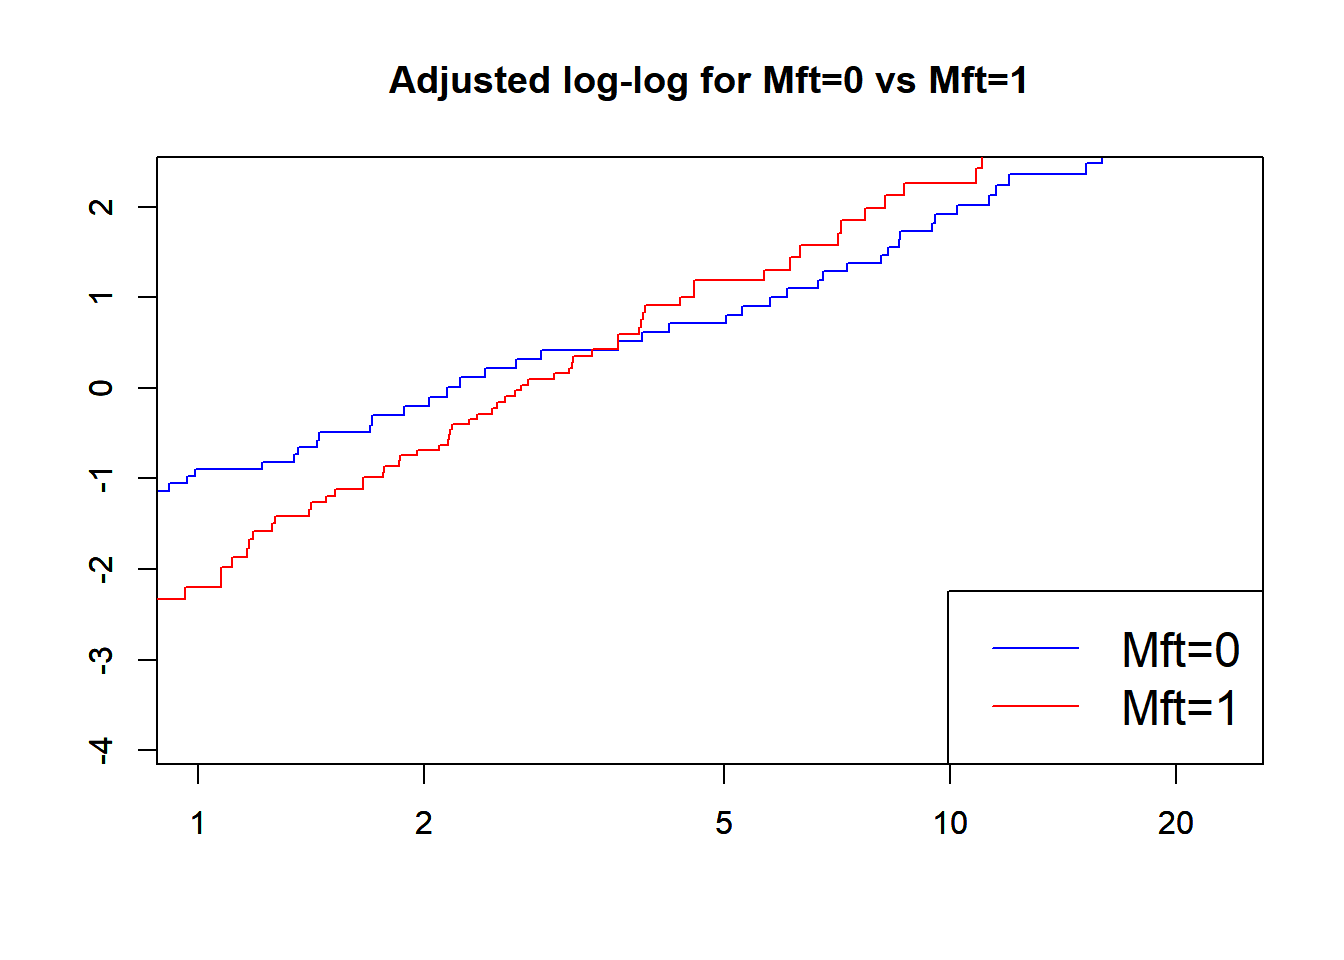
\includegraphics{HW4_629Solutions_files/figure-latex/unnamed-chunk-5-1.pdf}

\#3 Stratification by Mft

\begin{Shaded}
\begin{Highlighting}[]
\CommentTok{\#1 Fit a stratified model }
\NormalTok{Y}\OtherTok{\textless{}{-}}\FunctionTok{Surv}\NormalTok{(Ven.reset}\SpecialCharTok{$}\NormalTok{eventtime,Ven.reset}\SpecialCharTok{$}\NormalTok{status}\SpecialCharTok{==}\DecValTok{1}\NormalTok{)}
\NormalTok{coxph.Ven.m1}\OtherTok{\textless{}{-}}\FunctionTok{coxph}\NormalTok{(Y}\SpecialCharTok{\textasciitilde{}}\NormalTok{Setting }\SpecialCharTok{+}\NormalTok{ LO2 }\SpecialCharTok{+} \FunctionTok{strata}\NormalTok{(Mft),}\AttributeTok{data=}\NormalTok{Ven.reset)}
\FunctionTok{summary}\NormalTok{(coxph.Ven.m1)}
\end{Highlighting}
\end{Shaded}

\begin{verbatim}
## Call:
## coxph(formula = Y ~ Setting + LO2 + strata(Mft), data = Ven.reset)
## 
##   n= 150, number of events= 145 
## 
##            coef exp(coef) se(coef)      z Pr(>|z|)    
## Setting 0.96368   2.62133  0.12447  7.742 9.78e-15 ***
## LO2     0.83814   2.31206  0.07825 10.711  < 2e-16 ***
## ---
## Signif. codes:  0 '***' 0.001 '**' 0.01 '*' 0.05 '.' 0.1 ' ' 1
## 
##         exp(coef) exp(-coef) lower .95 upper .95
## Setting     2.621     0.3815     2.054     3.346
## LO2         2.312     0.4325     1.983     2.695
## 
## Concordance= 0.809  (se = 0.019 )
## Likelihood ratio test= 165.9  on 2 df,   p=<2e-16
## Wald test            = 131.7  on 2 df,   p=<2e-16
## Score (logrank) test = 155.1  on 2 df,   p=<2e-16
\end{verbatim}

Our fitted stratified Cox PH model is:
\(h(X,t)=h_0(t)\exp(0.96368*X_1+0.83814X_2)\).

\end{document}
